\chapter{实验评估}
\section{实验环境}
本次实验的环境为Windows 10 64位系统,CPU为四核Intel Xeon 3.3Ghz CPU,24G内存。代码开发环境为Python3.5和TensorfFow1.8.0版本。

TensorFlow是谷歌旗下的一款深度学习框架, 是一个使用数据流图进行数值计算的开放源代码软件库。利用TensorFlow框架可以轻松实现深度学习模型而不需要考虑算法的底层实现,并且TensorFlow提供多个优化器可供选择,其灵活的参数设置机制让使用者能够快速调整深度学习模型。因为其方便性与易用性,TensorFlow已经成为了机器学习工作者实现其模型的首选框架,这也是本文采用TensorFlow实现文中算法的原因。

\section{数据选择}

在第四章的数据集构建部分,总共生成了12780个用例。其中5340个用例为不含空指针引用缺陷的正常用例,7440个样例为包含空指针引用缺陷的用例。由于对于无缺陷的用例,四个工具大都能正常鉴别,区分度较小,所以在训练数据时限制了这些用例的数量,只是从这些用例中随机抽取1000个作为训练数据。对于包含空指针引用缺陷的用例,则需要去除掉一些控制流图节点数量异常和特征矩阵数据过于稀疏的用例。最终本文选取的训练集用例数量为8650个,对于这些数据,各个工具的检测结果已经在第三章的相关背景中的表\ref{fig:figure3-1}中给出。

如果直接将这批训练集放入模型训练的话,由于不同工具检测能力的差别,会导致标记的正负样本数量分布不均的情况,很容易出现模型直接收敛到样本多数值的问题,造成最终的模型泛化能力过低。为了解决样本分布不均的问题,本文试验了两种常用的方法,过采样和欠采样的方法。如图\ref{fig:caiyang}所示,过采样方法随机重复采样数量较少的样本,从而达到正负样本数量均衡的效果,不过重复的采样容易导致过拟合的问题。欠采样的方法随机丢弃一些多数样本的数据,在训练模型时保持正负样本数据数量的一致。

\begin{figure}[h]
	\label{fig:caiyang}
	\centering
	\subfigure [欠采样方法示例]{
		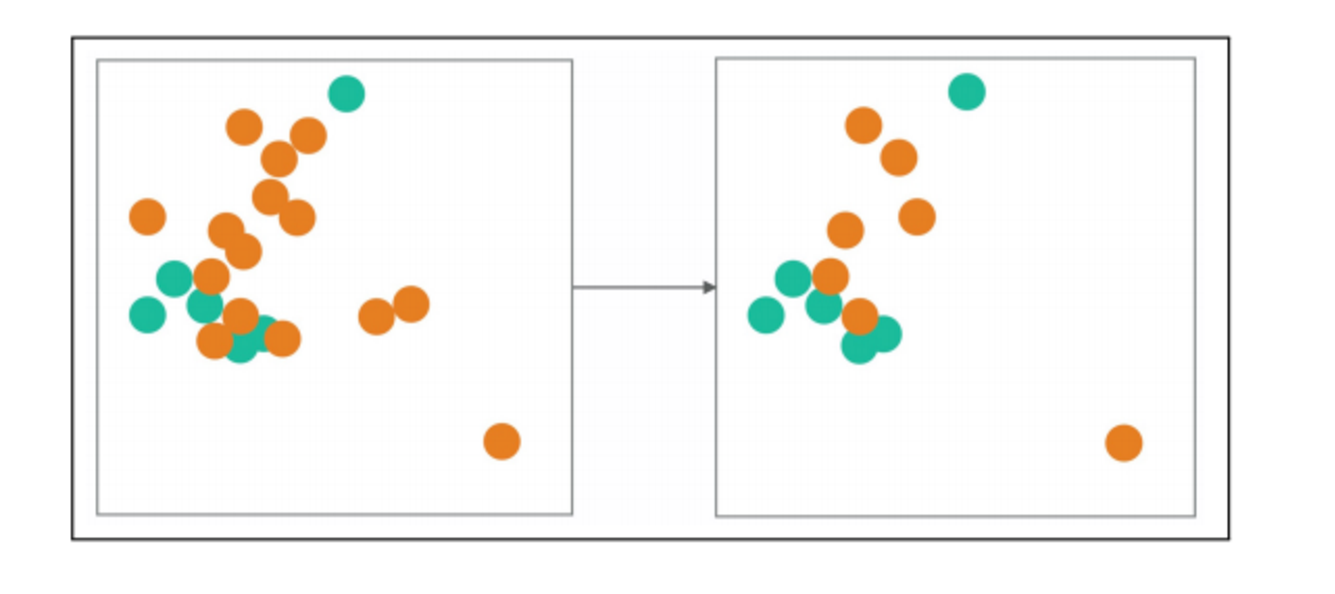
\includegraphics [width=0.45\textwidth]{figures/7}}
	\subfigure [过采样方法示例]{
		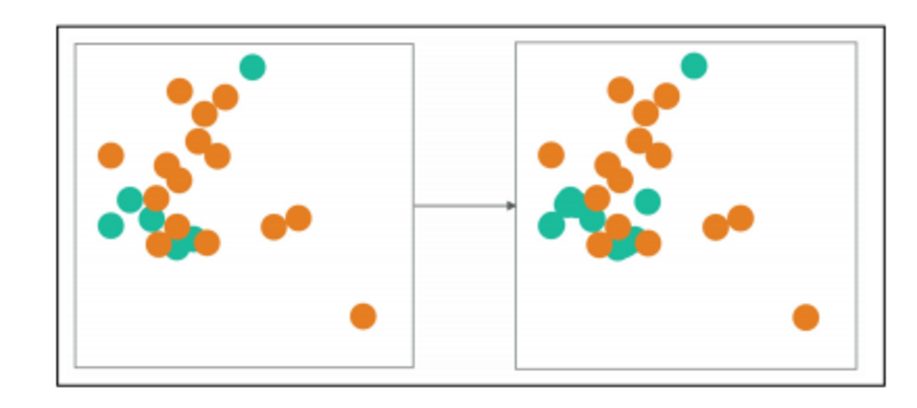
\includegraphics [width=0.45\textwidth]{figures/8}}
	\caption{两种采样方法示例}
\end{figure}

经过对比,本文选择了欠采样的方法。例如针对FindBugs工具,训练时在5834个检测正确的样本中随机挑选出1488个,与1488个缺陷样本一起加入训练,保证了训练数据正负样本的数量均衡。随机欠采样的方法既不会影响数据的统计特征,同时可以使正负样本的边界更为清晰。本文的测试数据采用了不同于训练数据的1000个代码样例,同样的,为了保证正负样本数量的均衡,每次测试时,本文从1000个样本中随机抽取正负样本各50个进行测试,测试十次得到测试的平均正确率。

\section{训练优化实验}
本次模型训练采用了TensorFlow的AdamOptimizer函数,AdamOptimizer实现了Adam优化算法,比起随机梯度下降的方法,Adam算法收敛速度更加迅速,陷入局部最优解的概率更小。当学习率过大时,容易导致模型发生振荡无法收敛,当学习率过小时,会导致模型收敛速度太慢耗时较长。为了避免上述情况的发生,本文采用了动态学习率的方法。训练学习率初始设置为$10^{4}$,学习率随着训练的迭代步数增加而呈阶梯状下降,每迭代100次降为原来的0.98倍。损失函数采用了交叉熵的算法。对两个概率分布$p$和$q$,通过$q$来表示$q$的交叉熵为:
$$H(p,q) = -\sum_x p(x)\log q(x)$$

通过交叉熵函数可以比较两个概率分布的差异。交叉熵越小,表示两个概率分布差异越小,优化器可以根据交叉熵的值更新模型参数。

针对本文提出的模型,有两个参数可能影响模型的结果:图压缩后特征向量的维度大小$d$以及压缩算法的迭代次数$T$。接下来将分别探讨两者的影响。


对于特征向量$d$,可以看出,当$d$的维度增加,网络中的参数$W_1, W_2, W_3, W_4$的维度都会相应的增加,相当于网络的每一层的神经元都会增加。网络变得更加复杂,能够拟合的函数也就越复杂。与此同时,模型的训练难度和时间消耗也会增加。网络如果过于复杂也有可能导致模型过拟合的问题。

对于循环次数$T$,相类似的,随着循环次数的增加,网络的层数逐渐增加,网络也会更加复杂,进而导致训练时长的增加和过拟合问题。

为了找到最佳的特征向量维度$d$以及迭代次数$T$,本文在迭代次数1到4次,特征维度8到512维之间分别进行了实验。实验采用了相同的训练数据,当模型收敛后对相同的测试集进行测试,得到四个分类器的准确率均值,结果如图\ref{mid}。由图可知,迭代次数为3,特征向量为32维时,训练效果最佳。
\begin{figure}[htbp]
	\begin{center}
		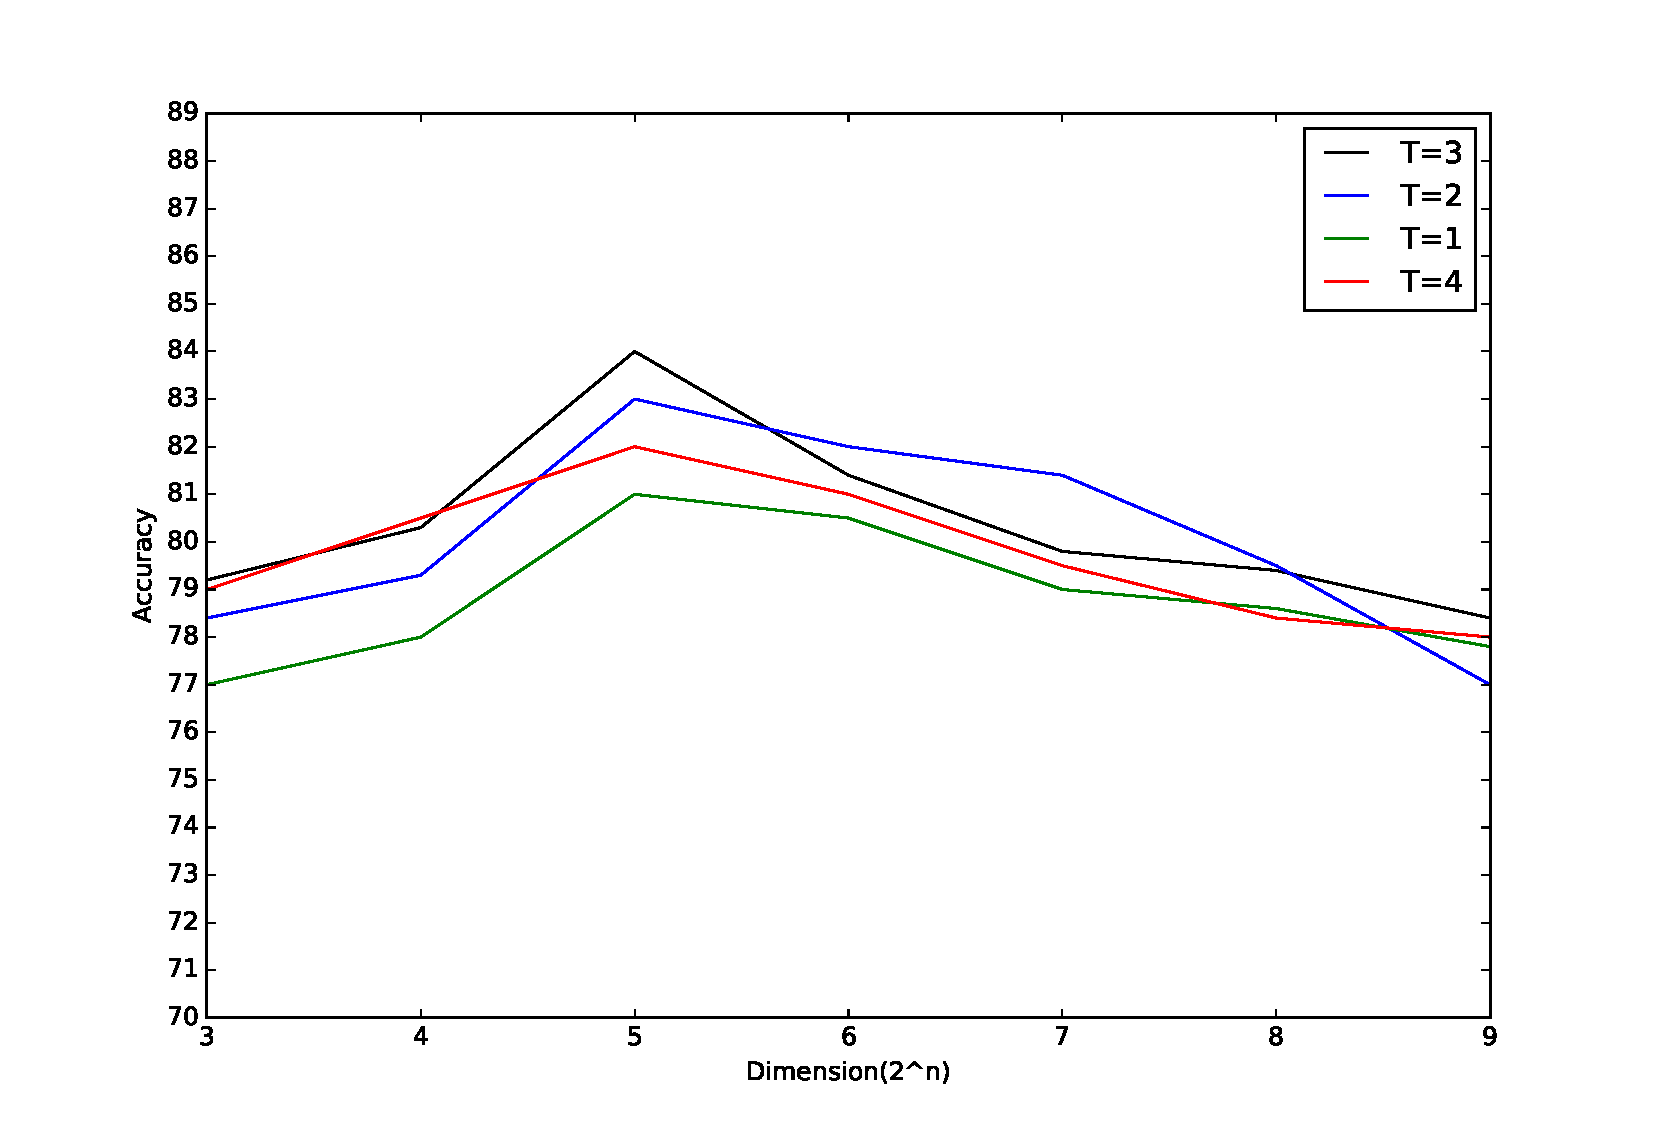
\includegraphics[width=0.95\textwidth]{figures/9.pdf}
		\caption{迭代次数和特征维度对模型训练的影响}
		\label{mid}
	\end{center}
\end{figure}
\section{模型检测实验}
在上文选择的训练集上进行训练之后,每一个工具都得到了一个二分类器,分类器在测试集上的分类准确率达到了80\%以上。为了让实验结果更加清晰,本文对模型产生的高维数据进行可视化。首先运用训练好的图特征抽取模型对测试代码控制流图进行向量化得到图特征向量,然后运用t-SNE算法将特征向量压缩为一个二维向量,根据各个工具对该代码检测结果的正确与否给该数据标记不同的颜色,得到了图\ref{fig:6-3}的结果。

\begin{figure}[h]
 \centering
 \subfigure [Findbugs]{
    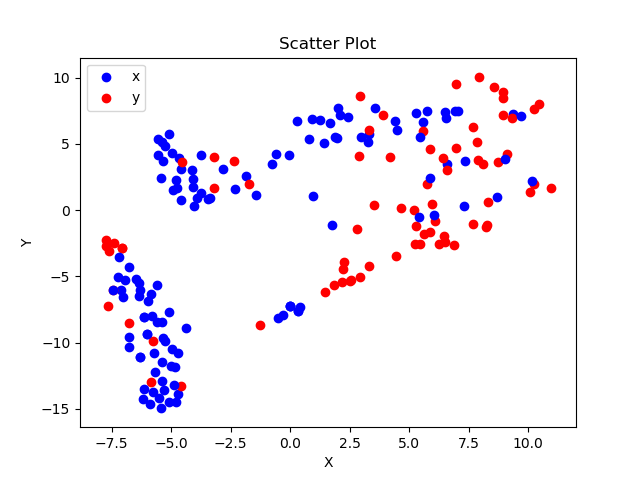
\includegraphics [width=0.45\textwidth]{figures/11}}
 \subfigure [Infer]{
    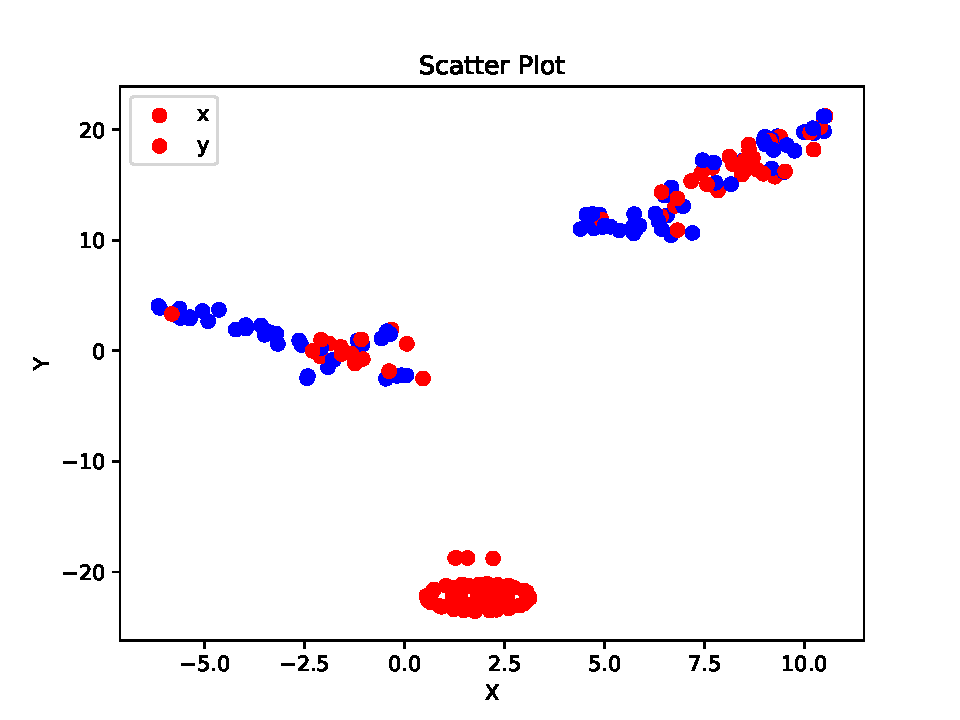
\includegraphics [width=0.45\textwidth]{figures/12}}
 \subfigure [Jlint]{
	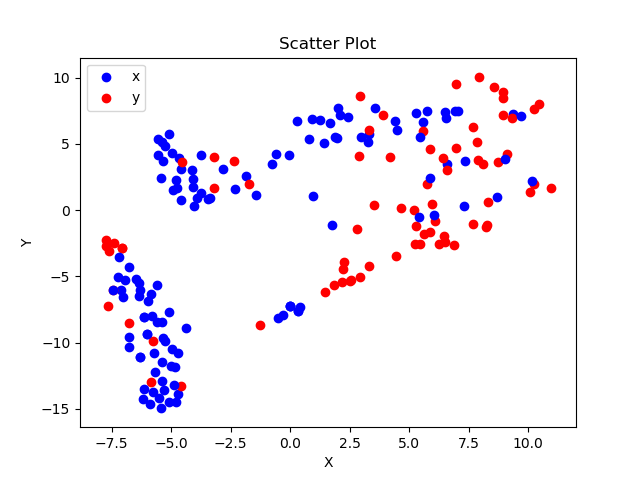
\includegraphics [width=0.45\textwidth]{figures/11}}
\subfigure [Fortify]{
	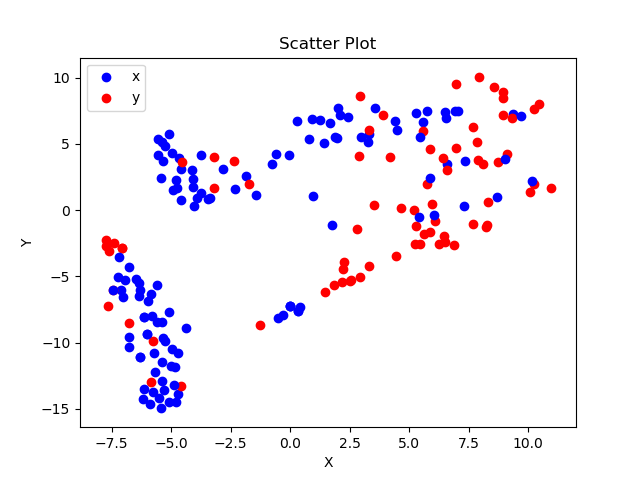
\includegraphics [width=0.45\textwidth]{figures/11}}
\label{fig:6-3}
 \caption{四种工具的二分类模型的分类效果}
\end{figure}

可以看出FindBugs的结果分布比较稀疏,说明了FindBugs的检测规则比较丰富,能够检测的代码类型较多;而其他三种工具的结果分布相比之下更聚集一些,说明其检测所需的特征比较单一,以该工具检测能力为标准对代码的分类更加明显。

同时,四个分类器的ROC曲线如图\ref{fig:6-4}所示:

\begin{figure}[ht]
	\label{fig:6-4}
	\centering
	\subfigure [Findbugs]{
		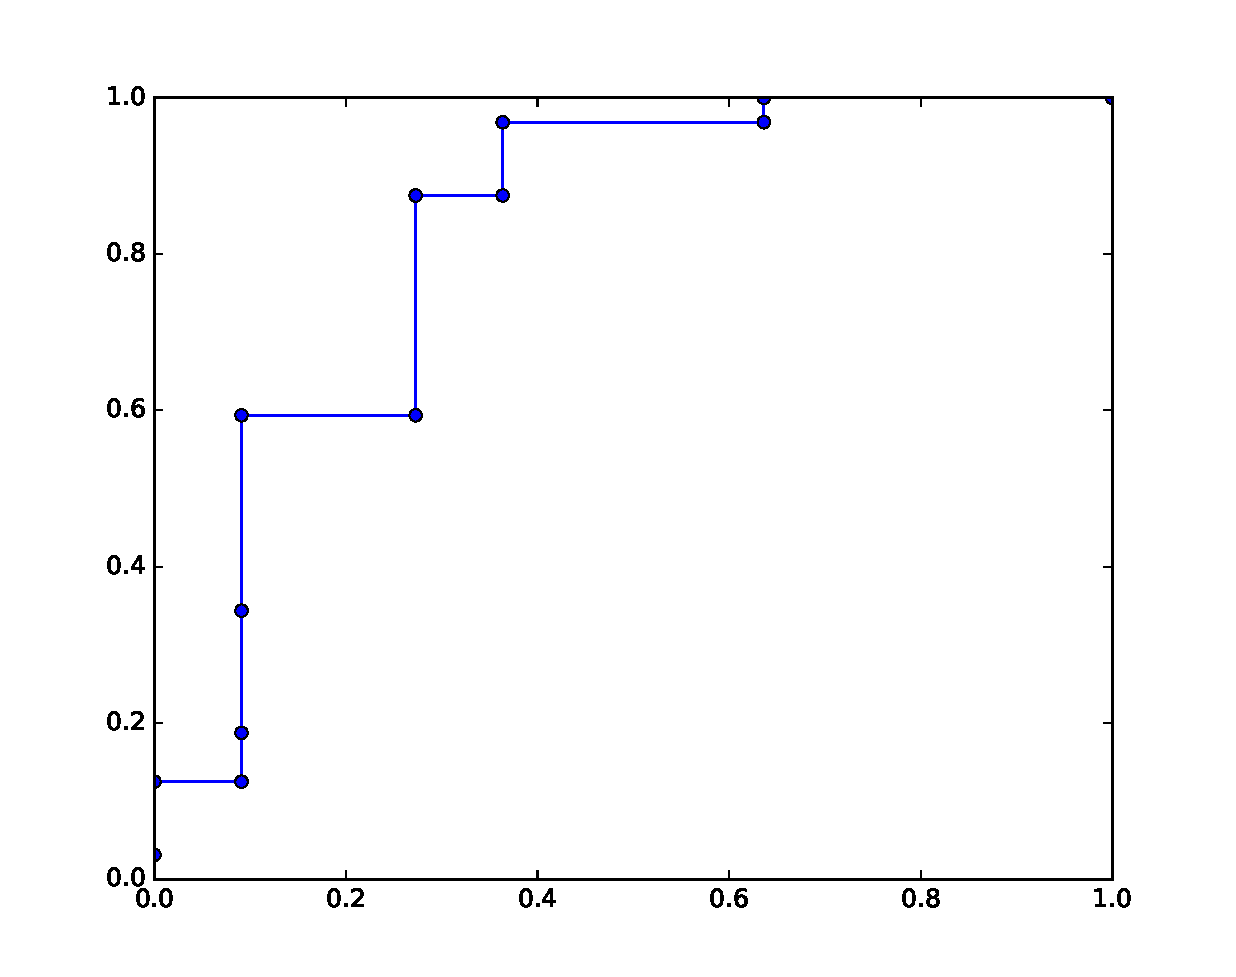
\includegraphics [width=0.45\textwidth]{figures/13}}
	\subfigure [Infer]{
		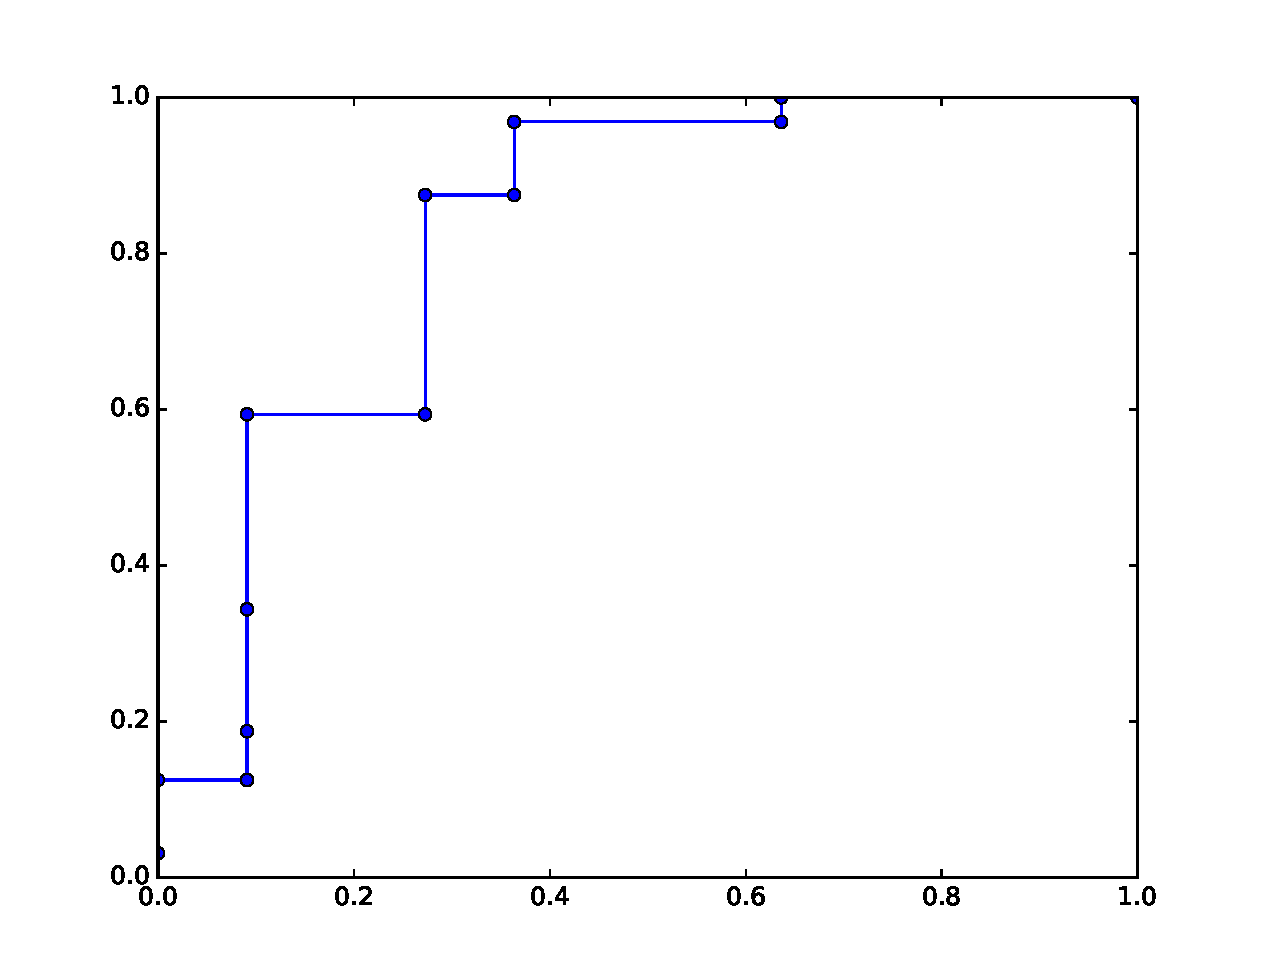
\includegraphics [width=0.45\textwidth]{figures/14}}
	\subfigure [Jlint]{
		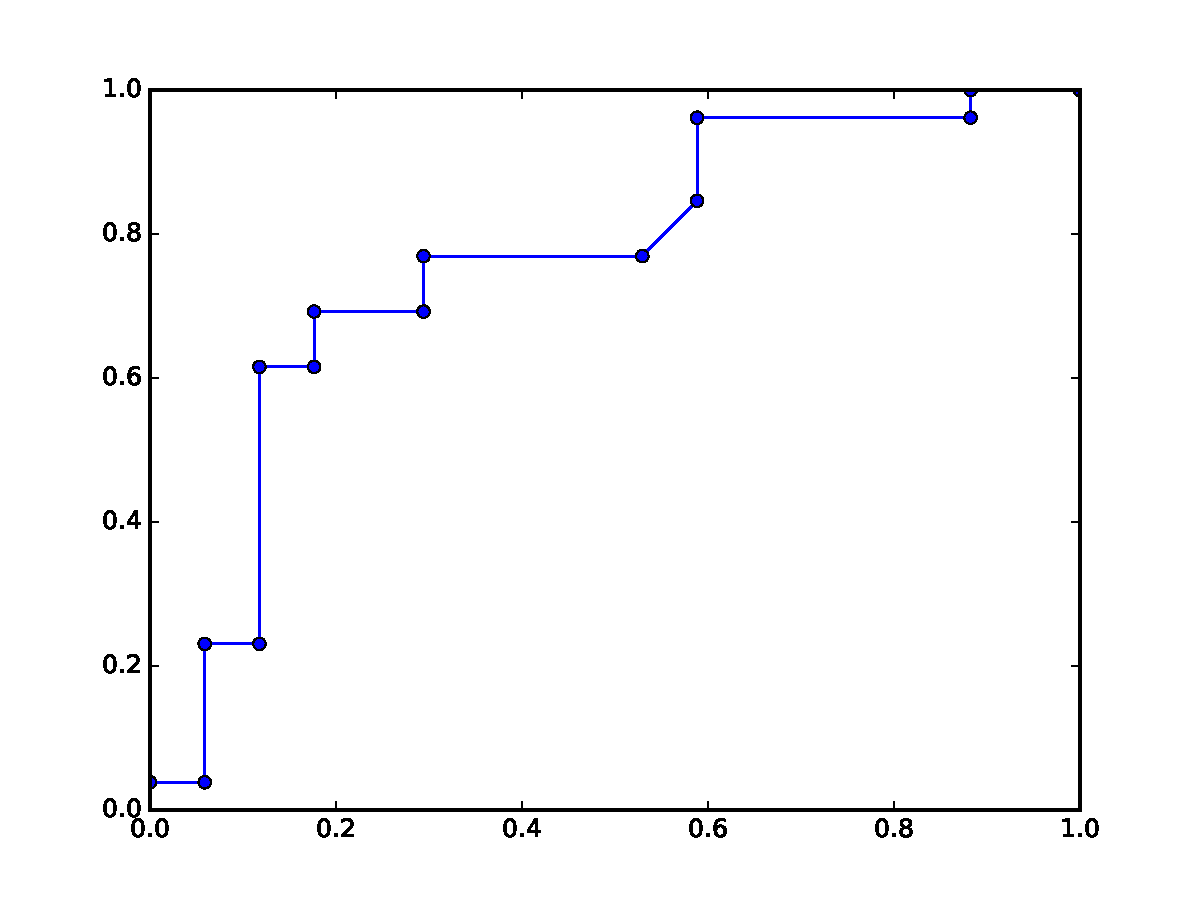
\includegraphics [width=0.45\textwidth]{figures/15}}
	\subfigure [Fortify]{
		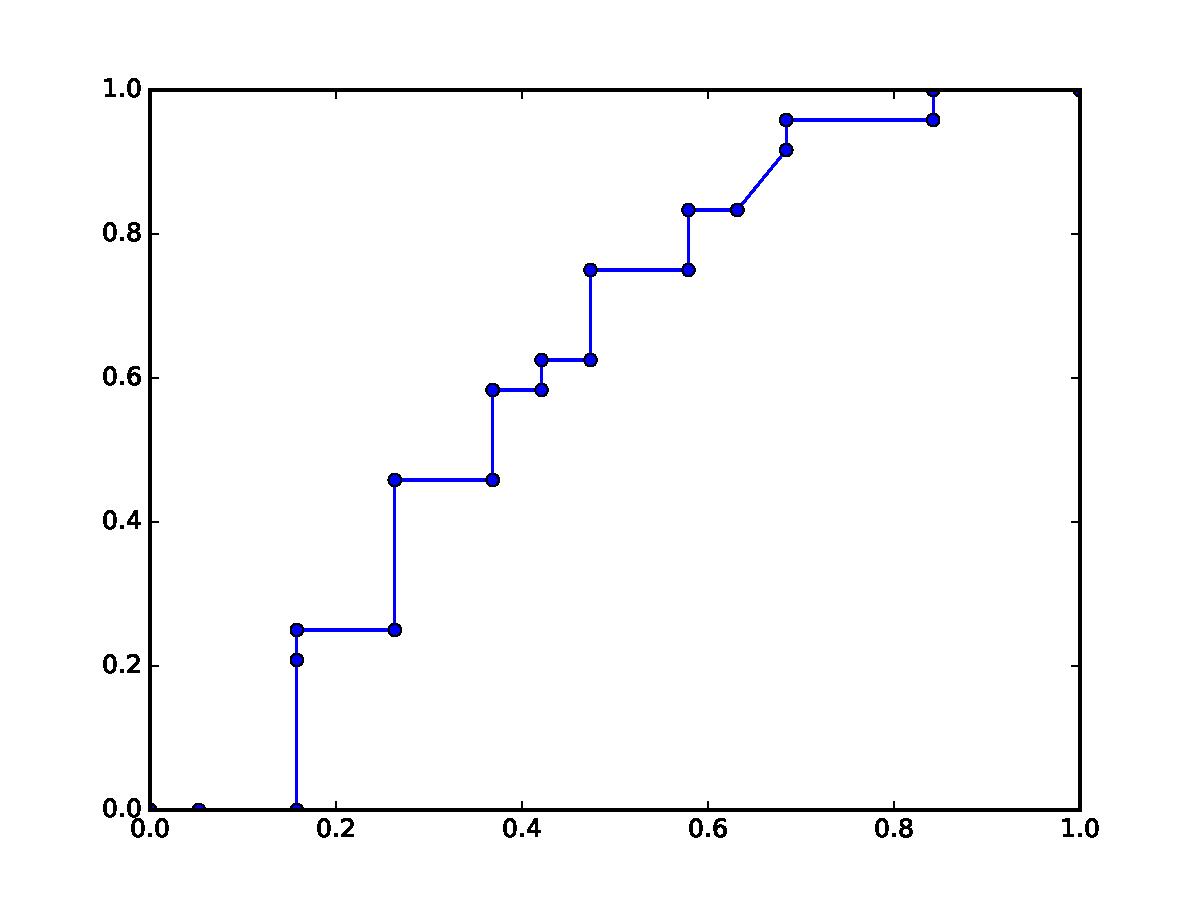
\includegraphics [width=0.45\textwidth]{figures/16}}
	\caption{四种工具的二分类模型的ROC曲线}
\end{figure}


得到四个工具对应的分类器后,可以综合分类模型预测的结果和工具的实际检测结果对用例产生缺陷的真实性进行判定。为了标识工具实际的检测结果,这里对数据标签进行再处理,当工具对测试用例实际能够检测出空指针引用缺陷时,该数据的标签置为1;当工具不能在该用例上检测出空指针缺陷时,标签置为0。这样就可以得到四个工具在一个用例上的检测结果向量$R={r_1, r_2, r_3, r_4}$,同时模型可以得到四个工具检测结果的置信度矩阵$W={w_1, w_2, w_3, w_4}$。则测试用例含有空指针引用缺陷的置信度为$P = W^T*R = \sum_{i=1}^4 w_i*r_i$。这样得到的结果具有一定的容错性,当一个分类器出现预测错误时,其他三个分类器的结果可以弱化此分类器的错误,从而最小化单个分类器的分类错误对整个判定模型的影响。为了实现对目标代码是否具有缺陷的最终判定,需要设定一个阈值$p$, 当$P>=p$时判定该代码存在空指针缺陷。

当模型分类完全没有误差时,阈值$p$应该接近于0。然而在现实中模型无法做到没有偏差,为了得到$p$最佳的取值,本文从-0.3到0.4,每隔0.05取一个阈值进行实验。实验从测试集中随机选取了1000个用例,使用这些数据对模型进行检验,计算缺陷判定准确率后得到图\ref{res}的结果:
\begin{figure}[ht]
	\begin{center}
		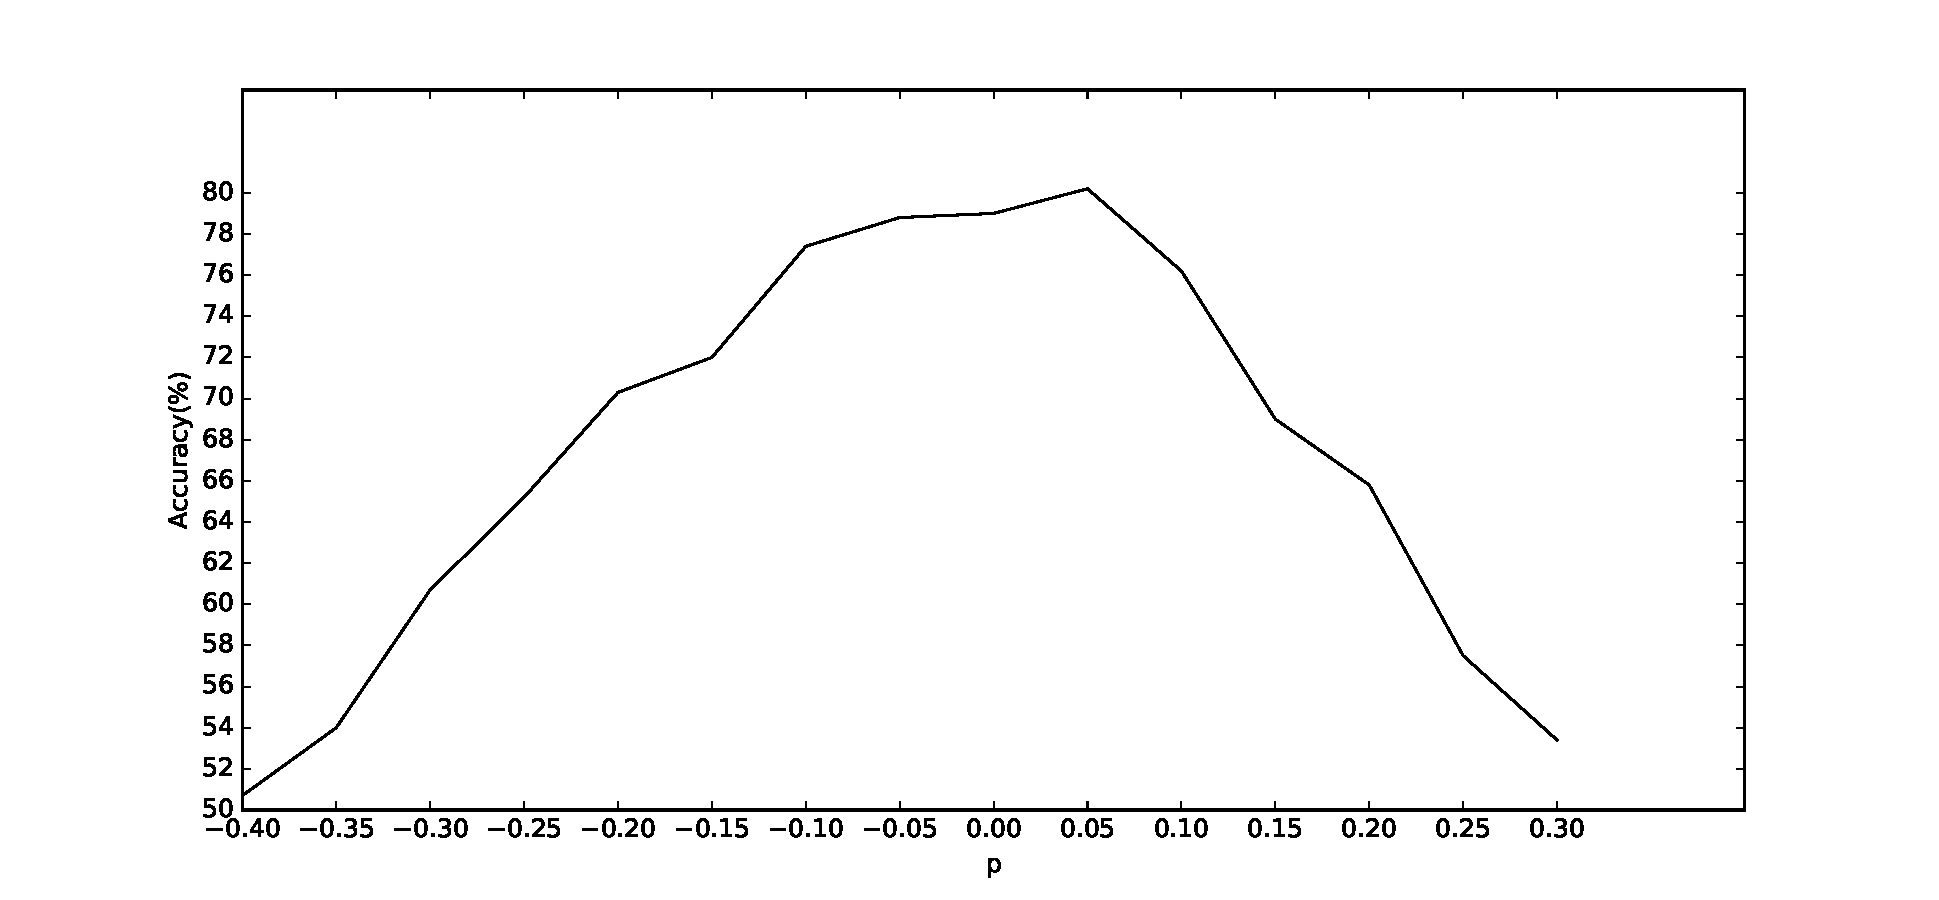
\includegraphics[width=0.95\textwidth]{figures//10.pdf}
		\caption{不同阈值下的缺陷判定准确率}
		\label{res}
	\end{center}
\end{figure}

可以看出,当阈值为0.05时能够取得最大的检测准确率81.34\%。然后,使用该阈值下的测试结果和在这些数据上不同工具的检测结果进行对比,可得表\ref{tt}。表中的BIT-Detector表示使用模型对所有缺陷进行验证得到的结果,可以看出,模型在综合了四种工具的检测结果置信度后,成功对工具检测的结果进行了修正,提高了检测的准确率。表中的BIT-Detector*只选取四种静态检测工具检测一致的结果作为输出,该部分结果的准确率依然最高,但这是用较高的漏报代价达到的。

虽然模型在工具已有检测结果的基础上利用代码分类可以给出更高的检测准确率,但是实验数据表明该准确率依然没有达到理想水平,不同工具能够同时检测的缺陷依然具有相当高的可信度。因此BIT-Detector使用可信度优先级排序的方式是最优解决方案,在不降低漏报率的前提下,报告靠前的部分拥有相对理想的可信度。后面的报告可以结合模型输出的缺陷置信度进行排序,这样排序的合理性能够得到保证,从而大幅提升检测报告的实用性。

\begin{table}[t]
	\centering
	\caption{训练集上工具检测结果}
	\label{tt}
	\begin{tabular*}{0.9\textwidth}{@{\extracolsep{\fill}}cccc}
		\toprule
		工具	&正确数量&错误数量&准确率	 \\
		\midrule
		FindBugs&760&240&76.0\%\\
		Infer&648&352&64.8\%\\
		Jlint&634&366&63.4\%\\
		Fortify&727&273&72.7\%\\
		BIT-Detector*&378&54&87.5\%\\
		BIT-Detector&813&187&81.3\%\\
		\bottomrule
	\end{tabular*}
\end{table}

\section{本章小结}

本章作为实验部分,首先对试验环境进行了介绍,并给出选择试验环境的原因。然后对模型训练和测试时选择的数据进行了介绍,随后对模型训练过程中的优化实验进行了分析,最后对模型的分类效果和最后预测效果进行了实验总结。